
\section{Le contexte de la gestion de projet}

\subsection{La notion de projet}

\frame{
\frametitle{Les origines}

\vspace{5mm}
\textbf{années 1950} : réflexion pour les grands projets industriels 
	(aéronautique, armement, travaux public)

\vspace{5mm}
\textbf{aujourd'hui} : projets de plus en plus importants (montants, internationalisation, ...)\\


\vspace{5mm}
\textbf{besoin de méthode} : constat d'échec et situation de crise
			(coûts, délais, non-fiabilité...) 

\vspace{5mm}
\textbf{influence organisationnelle} : certaines organisations
   se structurent en mode projet
\vfill
}
%*****************************************************************
\frame{\frametitle{Définition de la notion de Projet}

Un projet est une activité: 
\pause
\vspace{.2cm}
\begin{itemize}
\item<+-> unique et ponctuelle (non répétitive),\\
	    $\rightarrow$ 
	    \brown{date de début et fin du projet},
\vspace{.2cm}
\item<+-> soumise à des contraintes,\\
	    $\rightarrow$ 
	    \brown{de délais, coûts, qualité}.
\vspace{.2cm}
\item<+-> constituée d'actions ayant un objectif commun,\\
	    $\rightarrow$ 
	    \brown{nécessite des spécialistes aux compétences variées qu'il faut coordonner}, 
\vspace{.2cm}
\item<+-> qui produit un livrable\\
	    $\rightarrow$ 
	    \brown{résultat permettant la satisfaction d'un besoin identifié.}
\end{itemize}
}

%********************* Phases *************************************

\subsection{La genèse d'un projet}
\frame{\frametitle{Genèse d'un projet}


\begin{figure}[!htb]
\begin{tikzpicture}
[
      xscale      = 1,  % to scale horizontally everything but the text
      yscale      = 1,  % to scale vertically everything but the text
]

% Noeud "Besoin"
\node (besoin) [ 	shape             = circle,
            	top color         = white,        
            	bottom color      = blue!20!white, 
            	text              = blue,        
            	text width        = 1.4cm,        
            	align             = center,    
            	draw              = blue,     
            	rotate            = 2,       
            	thick,]
	at (-4,0) {Besoin};


%% --- etape 2
\only<2->{
% Noeud "Livrable"
\node (livrable) at (5,0)
	{
\includegraphics[height=1.7cm]{fig/livrable.png} Livrable};

% chemin 
\draw[dotted, ultra thick,->] (besoin) -- (livrable);
}


\onslide<3->{
\node (projet) [	shape             = rectangle,
            	top color         = white,
            	bottom color      = red!20!white, 	% |
            	text              = black,                % colour of the fonts
            	text width        = 3cm,        
            	align             = center,               % text alignment
            	draw              = red,                % colour of the border
            	align             = center,    
            	thick,]
		at (0,0) {Projet};
}

%% --- etape 4
\onslide<4->{
	\node (chefprojet) at (0,-2) {
\includegraphics[height=9mm] {fig/user_female.png}};
	\draw (0,-2.5) node[below]{{\small Chef de projet}};
	\draw[thick,->] (chefprojet) -- (projet);
}
\onslide<5->{
	\node (decideur) at (0,2) {
\includegraphics[height=9mm] {fig/user_executive.png}};
	\draw[thick,->] (decideur) -- (projet)
			    node[near start,above]{\small Décideur};
}
\onslide<6->{
	\node (equipe) at (2,-2) {
\includegraphics[height=9mm] {fig/user_group.png}};
	\draw (2,-2.5) node[below]{\small Equipes};
	\draw[thick,->] (equipe) -- (projet);
}
\end{tikzpicture}
\end{figure}
%  ______________________________________________________________________________________________
}


\subsection{La conduite du projet}
\frame{\frametitle{Conduite de projet}

La \emph{conduite de projet} est la façon dont cette démarche est menée.\\
\vspace{2cm}

C'est un cadre méthodologique qui préconise:
\begin{itemize}
\item<+-> les grandes phases d'un projet 
\item<+-> les étapes usuelles jalonnant un projet
\item<+-> les protocoles usuels entre les acteurs du projet
\end{itemize}
}

%********************* Phases *************************************
\frame{\frametitle{Les grandes phases}

\begin{itemize}
\item Définition
\item Réalisation
\item Mise en {\oe}uvre
\item Bilan 
\end{itemize}
}


%********************* Phases *************************************
\frame{
\begin{center}
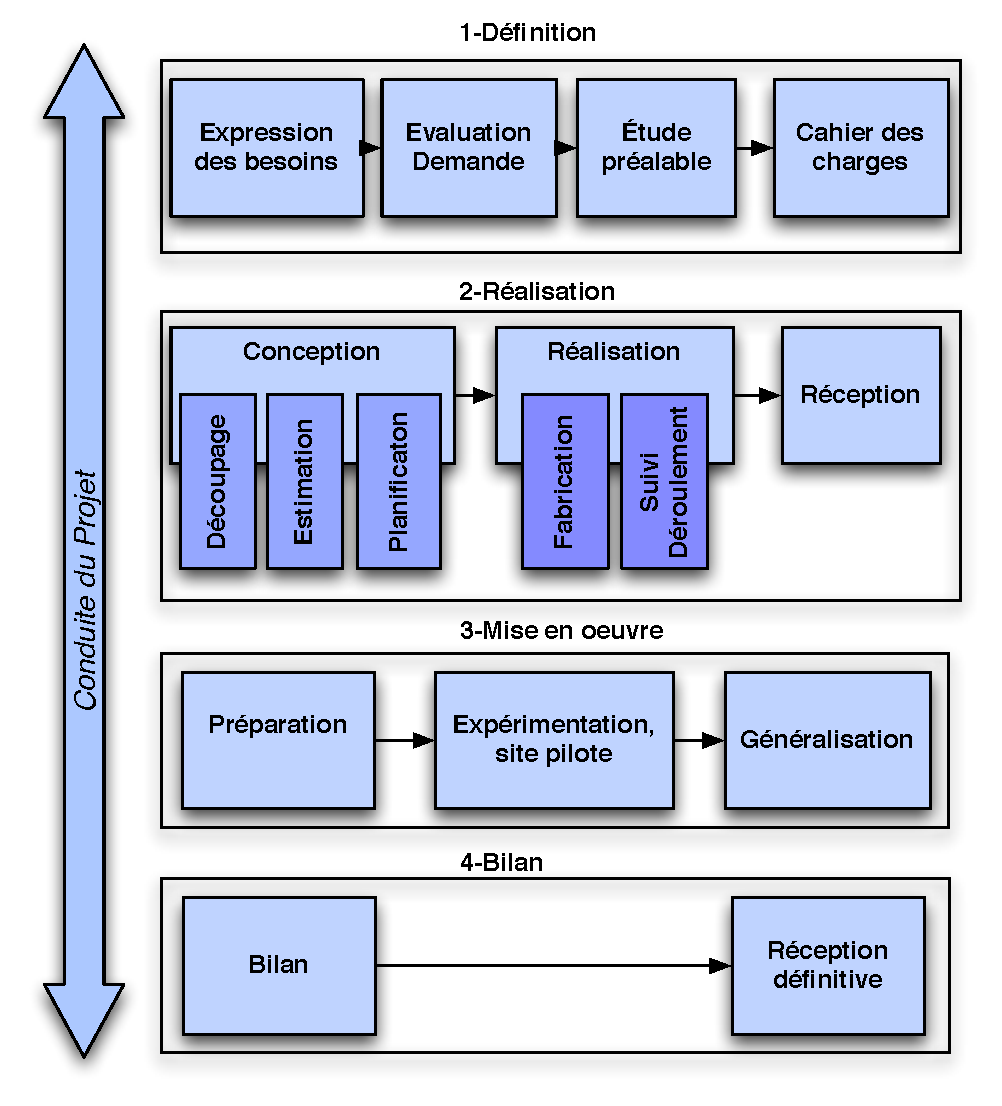
\includegraphics[height=\textheight]{overview-projet.pdf}
\end{center}
}


\subsection{Vérifier l'opportunité du projet}

%*****************************************************************
\frame{
\frametitle{Etude d'opportunité}

\onslide<1>{\center ... Avant de se lancer ...}
\pause
\begin{figure}[!htb]
\begin{tikzpicture} [xscale=1,yscale=1]

% Noeud "Besoin"
\node (besoin) [ 	shape             = circle,
            	top color         = white,        
            	bottom color      = blue!20!white, 
            	text              = blue,        
            	text width        = 1.4cm,        
            	align             = center,    
            	draw              = blue,     
            	rotate            = 2,       
            	thick,]
	at (-4,0) {Besoin};

\node (livrable) at (5,0)
	{
\includegraphics[height=1.7cm]{fig/livrable.png} Livrable};
\draw[dotted, ultra thick,->] (besoin) -- (livrable);
\node (projet) [	shape             = rectangle,
            	top color         = gray!20!white,
            	bottom color      = red!20!white, 	% |
            	text              = black,                % colour of the fonts
            	text width        = 3cm,        
            	align             = center,               % text alignment
            	draw              = red,                % colour of the border
            	align             = center,    
            	thick,]
		at (0,0) {Projet};

\node (opportunite) [shape             = rectangle,
            	top color         = white,        
            	bottom color      = red!20!white, 	% |
            	text              = black,                % colour of the fonts
            	text width        = 2cm,        
            	align             = center,               % text alignment
            	draw              = red,                % colour of the border
            	align             = center,    
            	thick,]
		at (-1.5,-1.5) {\'Etude opportunité};
\draw[ultra thick,->] (opportunite) -- (-1.8,-.1);


\end{tikzpicture}
\end{figure}
}
%  ______________________________________________________________________________________________



%*****************************************************************
\frame{
\frametitle{Etude d'opportunité}


\vspace{.5cm}
Avant acceptation ou lancement, se poser des questions :\\ 

\vspace{.5cm}
Toute difficulté identifiée devra faire l'objet 
d'un dialogue approfondi avec le demandeur pour

\begin{itemize}
\item soit annuler, infléchir ou différer le projet
\item soit négocier des moyens de réussite à hauteur des enjeux et des conditions de
réussite identifiées.
\end{itemize}

\vspace{.5cm}
$\Rightarrow$ Une \underline{évaluation} 
sous différents angles est nécessaire.
}

\frame{
\frametitle{Exemple simple: l'électricien}

\begin{block}{La demande}
Le client veut un site web pour 
\begin{itemize}
\item informer ses clients (horaires, produits, services, ...),
\item enregistrer demandes de devis, 
\item distribuer un dépliant electronique, 
\item ...
\end{itemize}
\end{block}
}

\frame{
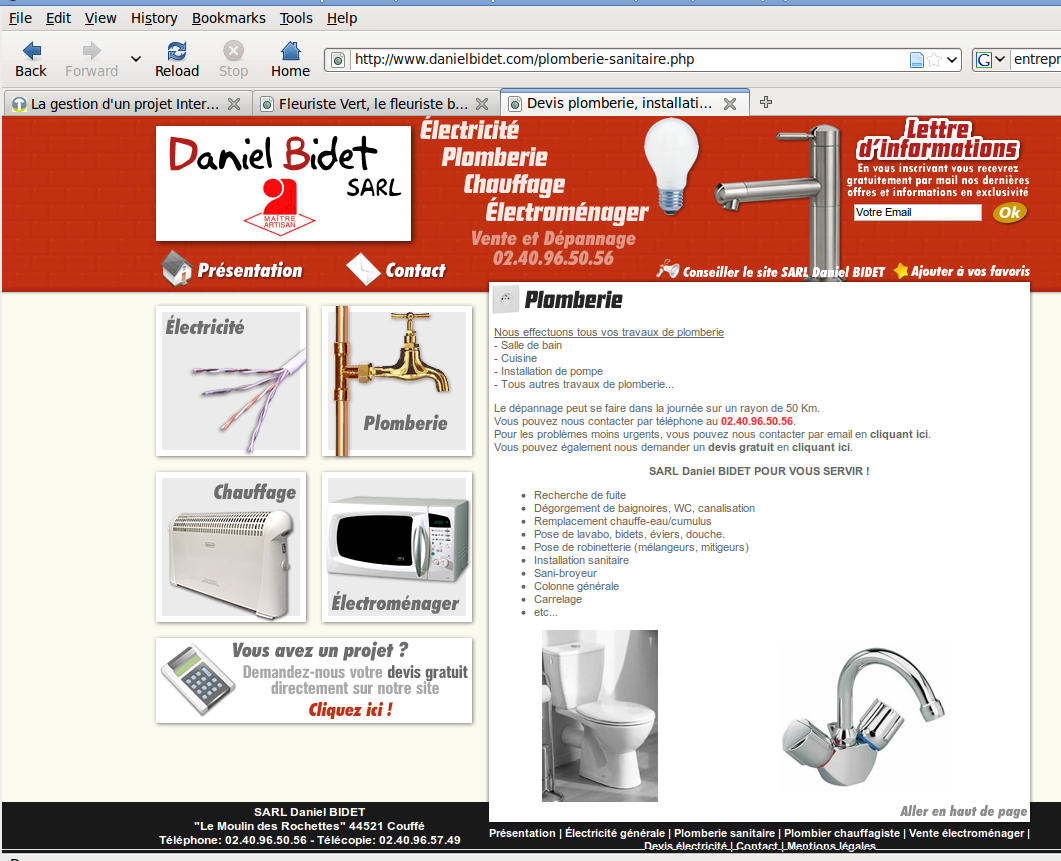
\includegraphics[width=\textwidth]{capture-site-electr.png}
}

\frame{
\frametitle{Exemple simple: l'électricien}

\begin{block}{La demande}
Le client veut un site web pour 
\begin{itemize}
\item informer ses clients (horaires, produits, services, ...),
\item enregistrer demandes de devis, 
\item distribuer un dépliant electronique, 
\item ...
\end{itemize}
\end{block}

\only<1>{Simple, non ? ...}
\only<2>{... Pourtant, répondre à cette demande nécessite de dialoguer avec le client.}

}
\frame{
\textit{
Quelques questions immédiates (liste non-exhaustive):
\begin{itemize}
    \item<+-> Qui décidera des informations nouvelles à enregistrer et publier ?
    \item<+-> Sur quels critères mettra t-on les informations produits/tarifs à jour ?
    \item<+-> De qui et comment viendront ces informations ?
    \item<+-> Qui mettra ces informations en ligne, sous quelle forme ? 
    \item<+-> Quelles compétences sont requises pour intervenir sur le site ? 
    \item<+-> Les visiteurs auront-ils le moyen d'enregistrer des alertes ? 
    \item<+-> Qui sera alerté ? Avec quels critères ? 
    \item<+-> ... Un deuxième niveau de questions devra cerner les motivations des acteurs...
\end{itemize}
}

\vspace{5mm}
\onslide<9->{Risque: un site au contenu périmé \ding{63} }
\onslide<10>{$\Rightarrow$ Adopter une démarche d'évaluation: le projet est-il clairement défini ?}
}

%*****************************************************************
\subsection{Lancement du projet: l'évaluation }
\frame{
\frametitle{Lancement du projet: l'évaluation}

Entre l'idée et sa réalisation, il peut y avoir un gouffre.
Le résultat attendu peut être flou et les implications mal cernées.  

\begin{block}{Règle 1 : Définissez l'idée en termes de résultat attendu}
    S'assurer que les décideurs sont d'accords avec ces résultats et peuvent dire ce qui va changer par rapport à ce qui est connu.

\pause
    \begin{itemize}
    \item<+-> Tous les acteurs ont ils la même représentation du produit attendu ?
    \item<+-> Cerner la demande : demande énoncée clairement, nature de la demande, cadre de la demande, les délais 
    \item<+-> Quels changements l'idée va t-elle produire ? Sont ils acceptables dans les structures et comportements ?
Que faut il faire pour les rendre acceptables ? 
    \end{itemize}
\end{block}  
}



\frame{
\frametitle{Evaluer le projet}

Le résultat attendu peut être ``contre-nature''.

\begin{block}{Règle 2 : évaluer la cohérence} 
Evaluer par la cohérence du projet dans le contexte de l'organisation
    \begin{itemize}
    \item<+-> Identifier le demandeur et protagonsites impliqués (initiateur, décideur, destinataire)
		% Ex: la demande vient des utilisateurs d'un service, relayée par le responsable du service,
		% appuyée par le chef du département et avalisée par la direction
    \item<+-> Générateur de résultats économiques ?
		% Va t-on avoir des gains ? quantifiables ?
    \item<+-> Les résultats escomptés sont ils en accord avec la stratégie de l'entreprise ? 
		% pas de contradiction avec les objectifs généraux affichés
		% Ex: l'entreprise annonce qu'elle passe d'une distrib. par revendeurs à distrib. directe mais le projet
		% concerne l'amélioration de la logistique de livraison des revendeurs
    \item<+-> Le projet s'inscrit-il dans la planification générale de l'entreprise ?
    Positionnement vis-à-vis d'autres projets ou actions ? (antinomies, synergies, compétition )
		% Ex: le projet logistique permet de livrer et d'informer les distributeurs sur les nouveaux produits mais
		% parallèlement un projet d'extranet revendeurs fournira également un catalogue et infos produits
    \end{itemize}
\end{block}
}


\frame{
\frametitle{Evaluer le projet }

Le projet peut devenir incontrôlable.

\begin{block}{Règle 3 : évaluer la conduite de projet} 
Evaluer par la conduite de projet : les risques d'aléas
    \begin{itemize}
    \item <+-> Garanties de progression et d'achèvement ? 
    \item <+-> Programme des étapes et décisions intermédiaires connus ?
    \item <+-> Les indicateurs de bonne fin sont ils précisés ?
    \end{itemize}
	
\end{block}
}

%******** CAS Personal Fit  ***************************
\frame{
\frametitle{Cas \textit{Personal Fit}}

\textbf{4.5.6} est une enseigne de prêt à porter pour femme, dont la cible est
la clientèle 30-50 ans. La marque est présente sous la forme d'un réseau de
franchisés (95 boutiques).

\pause
%\vskip
Sa direction est organisée comme suit:

\begin{figure}[!htb]
\begin{tikzpicture} [xscale=1,yscale=1]
\onslide<2->{
	\node (pdg) at (-5,0) {
\includegraphics[height=12mm] {fig/user_executive.png}};
	\draw (-5,-.75) node[below]{{\footnotesize PDG}};
}
\onslide<3->{
	\node (daf) at (-3,0) {
\includegraphics[height=12mm] {fig/exec_green_user.png}};
	\draw (-3,-1.25) node[below]{{\footnotesize DAF}};
}
\onslide<4->{
	\node (dp) at (-0.5,0) {
\includegraphics[height=12mm] {fig/registered_user.png}};
	\draw (-0.5,-.75) node[below]{{\footnotesize Dir. Production}};
}
\onslide<5->{
	\node (dp) at (2.5,0) {
\includegraphics[height=12mm] {fig/user_female2.png}};
	\draw (2.5,-1.25) node[below]{{\footnotesize Dir. Commerciale}};
}
\onslide<6->{
	\node (codir) at (5,0) {
\includegraphics[height=15mm] {fig/user_group.png}};
	\draw (5,-.75) node[below]{{\footnotesize Comité de Direction}};
}
\end{tikzpicture}
\end{figure}
%******** CAS 

\onslide<7->{
\begin{block}{}
4.5.6 désire lancer une offre distinctive \textit{Personal Fit}, un service de
vêtements ``sur mesure`'': une gamme spécifique de vêtements avec un choix de tailles
beaucoup plus fin, qui peut être guidé par des mesures electroniques. 
\onslide<8>{\ldots \textbf{voir étude de cas} \ldots}
\end{block}
}
}

%____________________________ L E S   A C T E U R S __________________________________

\section{Les acteurs}

\subsection{La défintion du projet}

\frame{
\frametitle{La définition du projet}

Le projet est fortement personnalisé par le \emph{chef de projet}.
\vspace{1cm}

\pause
Dans notre exemple de la société 4.5.6, le chef de projet dépend de la direction
commerciale .

\begin{figure}[!htb]
\begin{tikzpicture}
 	\node(chefprojet) at (-1,0) {
\includegraphics[height=9mm] {fig/user_female.png}};
	\node(dircommerciale) at (1,0) {
\includegraphics[height=9mm] {fig/user_female2.png}};
	\draw[->,ultra thick] (chefprojet) -- (dircommerciale);
\end{tikzpicture}
\end{figure}
\pause

C'est lui qui va \textbf{définir} le projet: 
\begin{itemize}
\item définir l'objectif : livrable, périmètre, ...
\item négocier les moyens
\item négocier les délais
\end{itemize}
}


\subsection{Le triangle projet: objectifs, délais, ressources}


%*****************************************************************
\frame{
\frametitle{Le triangle projet}

Pour le chef de projet:

\begin{figure}[!htb]
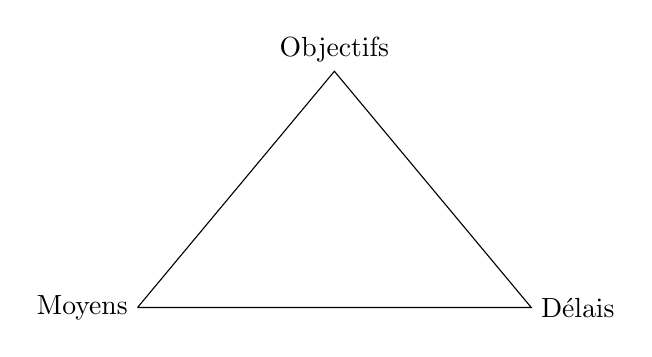
\begin{tikzpicture} [xscale=1,yscale=1]
	\draw (-2.5,-1) 	node[left]{Moyens}  -- 
	      (2.5,-1)  	node[right]{Délais} -- 
		(0,2)   	node[above]{Objectifs} -- 
	      (-2.5,-1);
\end{tikzpicture}
\end{figure}
}


\frame{
\frametitle{Les objectifs}

\begin{center}
	`` Quoi faire ? ''
\end{center}

Définir le domaine couvert en termes de \textbf{fonctionnalités} 
et de \textbf{qualité}. 

Le document contractuel est le \alert{cahier des charges}.
}

\frame{
\frametitle{Les délais}
\begin{center}
	`` Quand faire ? ''
\end{center}
La gestion des délais intervient une fois les étapes de découpage et d'estimation terminées. 
Un \alert{calendrier} contractuel définissant les délivrables intermédiaires peut être établi.
}

 
\frame{
\frametitle{Les ressources}

\begin{center}
	`` Avec qui/quoi faire ? ''
\end{center}

Une fois l'activité définie, il faut prévoir des \alert{ressources}
pour les réaliser.
}

%******************************************************************
\subsection{Le chef de projet au centre}

\frame{
\frametitle{Le chef de projet au centre}

\begin{figure}[!hbt]
\begin{tikzpicture}

% Noeud "Besoin"
\node (cercle) [ 	shape             = circle,
            	top color         = white,        
            	bottom color      = gray!20!white, 
            	text width        = 5cm,        
            	draw              = black,     
            	thick,]
	at (0,0) {};

\node (chefprojet) at (0,0) {
\includegraphics[height=9mm] {fig/user_female.png}};

\onslide<2->{
	\node (decideur) at (0,2) {
\includegraphics[height=9mm] {fig/user_executive.png}};
	\draw[thick,->] (decideur) -- (projet)
			    node[near start,above]{\small Décideur};
	\node (utilisateurs) at (1.5,3) {
\includegraphics[height=9mm] {fig/user_group.png}};
	\draw (1.5,3.5) node[below]{\small Utilisateurs};
	\draw[thick,->] (utilisateurs) -- (decideur);
	\draw[thick,->] (utilisateurs) -- (chefprojet);
}

\onslide<3->{
	\node(dircommerciale) at (-2.3,-2.3) {
\includegraphics[height=9mm] {fig/user_female2.png}};
	\draw (-2.2,-2.8) node[below]{\small Hiérarchie};
	\draw[->,thick] (dircommerciale) -- (chefprojet) ;
}
\onslide<4->{
	\node (equipe) at (2,-2) {
\includegraphics[height=9mm] {fig/user_group.png}};
	\draw (2,-2.5) node[below]{\small Equipes};
	\draw[thick,->] (equipe) -- (projet);
}
\end{tikzpicture}
\end{figure}
}
%  ______________________________________________________________________________________________

\subsection{La maîtrise d'{\oe}uvre (MOE)}
\frame{
\frametitle{La maîtrise d'{\oe}uvre (MOE)}

\begin{itemize}
\item<+-> Le chef de projet ne peut pas tout faire tout seul.
\vspace{5mm}
\item<+-> Le maître d'{\oe}uvre (MOE) est en charge des aspects opérationnels.
\vspace{5mm}
\item<+-> Il a une vision d'ensemble de l'utilisation des ressources.
\vspace{5mm}
\item<+-> Il arbitre les priorités entre les différents projets et
les autres activités.
\vspace{5mm}
\end{itemize}

}

\frame{
\frametitle{Le maître d'{\oe}uvre}

\begin{figure}[!hbt]
\begin{tikzpicture}

% Noeud "Besoin"
\node (cercle) [ 	shape             = circle,
            	top color         = white,        
            	bottom color      = gray!20!white, 
            	text width        = 5cm,        
            	draw              = black,     
            	thick,]
	at (0,0) {};

\node (chefprojet) at (0,0) {
\includegraphics[height=9mm] {fig/user_female.png}};

	\node (decideur) at (0,2) {
\includegraphics[height=9mm] {fig/user_executive.png}};
	\draw[thick,->] (decideur) -- (projet)
			    node[near start,above]{\small Décideur};
	\node (utilisateurs) at (1.5,3) {
\includegraphics[height=9mm] {fig/user_group.png}};
	\draw (1.5,3.5) node[below]{\small Utilisateurs};
	\draw[thick,->] (utilisateurs) -- (decideur);
	\draw[thick,->] (utilisateurs) -- (chefprojet);

	\node(dircommerciale) at (-2.3,-2.3) {
\includegraphics[height=9mm] {fig/user_female2.png}};
	\draw (-2.2,-2.8) node[below]{\small Hiérarchie};
	\draw[->,thick] (dircommerciale) -- (chefprojet) ;

	\node (moe) at (1.7,-1.7) {
\includegraphics[height=9mm] {fig/registered_user.png}};
	\draw (1.7,-2) node[below]{\small \alert{MOE}};
	\draw[thick,<->] (moe) -- (projet);

	\node (equipe) at (3,-3) {
\includegraphics[height=9mm] {fig/user_group.png}};
	\draw (3,-3.5) node[below]{\footnotesize Ressources};
	\draw[thick,-] (moe) -- (equipe);


\end{tikzpicture}
\end{figure}
}
%  ______________________________________________________________________________________________



\frame{
\frametitle{Structuration client/fournisseur}

Dans de nombreux projets, on peut retrouver les acteurs suivants:

\underline{parmi les clients} :
\begin{itemize}
\item les décideurs
\item le chef de projet
\item les usagers
\end{itemize}

\underline{parmi les fournisseurs} :
\begin{itemize}
\item le chef de projet
\item les concepteurs
\item les équipes de fabrication
\end{itemize}
\vfill
}
%******************************************************************

\subsection{Structuration maîtrise d'ouvrage/maîtrise d'{\oe}uvre}
\frame{
\frametitle{Structuration maîtrise d'ouvrage/maîtrise d'{\oe}uvre}

Quand les entreprises sont structurées pour gérer des projets 
on a souvent une organisation en \textbf{maîtrise d'ouvrage} (MOA) et
 \textbf{maîtrise d'{\oe}uvre} (MOE).\\

\pause
Ce sont deux entités de l'organisation (personnes morales).
\pause

\begin{itemize}
\item<+-> Le MOA est client du MOE à qui il passe commande d'un produit nécessaire à son activité.
\item<+-> Le MOE fournit ce produit: soit il le réalise lui-même, soit il passe commande à un ou plusieurs fournisseurs qui élaborent le produit sous sa direction. 
\end {itemize} 

}

\frame{
\frametitle{Les acteurs : structuration}
\input{acteurs.pdftex_t}

}   
\frame{
\frametitle{La maîtrise d'ouvrage : 6 fonctions}
\begin{itemize}
\item<+-> le maître d'ouvrage stratégique (MOAS)\\
	$\rightarrow$ prend les décisions, arbitre.
\item<+->  le maître d'ouvrage délégué (MOAD)\\
	$\rightarrow$ fournit les éléments factuels au MOAS.
\item<+->  le maître d'ouvrage opérationnel (MOAO)\\
	$\rightarrow$ expert d'un grand processus du métier.
\item<+->  l'assistant à maîtrise d'ouvrage (AMO),\\
      $\rightarrow$ support pour le MOAO ou MOAD en période de pointe, ou quand le projet demande des compétences non maitrisées. 
\item<+->  l'expert métier,\\
      $\rightarrow$ vérifie la pertinence du produit avec les exigences des utilisateurs
\item<+->   l'utilisateur\\
       $\rightarrow$ peuvent compléter les observations de l'expert métier.
\end {itemize}

}

\frame{
\frametitle{La maîtrise d'{\oe}uvre}

Le MOE est responsable de la qualité technique de la solution. 
Il doit, avant toute livraison au MOA, 
procéder aux vérifications nécessaires (``recette usine'').\\

\vspace{1cm}
 
Pour cela, le MOE doit assurer la coordination de tous les fabriquants en veillant (entre autres):
\begin{itemize}
\item à la cohérence des fournitures et à leur compatibilité,
\item à coordonner l'action des fournisseurs en contrôlant la qualité technique,
\item à respecter les délais fixés par le MOA et en minimisant les risques.
\end{itemize}
}


%*****************************************************************
\subsection{Des intérêts antagonistes}
\frame{
\frametitle{Des intérêts antagonistes}
\begin{columns}
%-- col1
\begin{column}{.45\textwidth}
\onslide<4->{
	Le client:
	\begin{itemize}
	\item augmenter la valeur pour les utilisateurs
	\item diminuer les coûts
	\item sans prendre de risque
	\end{itemize}
}
\vspace{5mm}
\onslide<2->{
	Le chef de projet:
	\begin{itemize}
	\item maintenir la conformité
	\item respecter le budget
	\item respecter les délais
	\end{itemize}
}
\end{column}
%-- col2
\begin{column}{.55\textwidth}
\begin{figure}[!htb]
\begin{tikzpicture} [xscale=.5,yscale=.5]


\onslide<3->{
	\node (decideur) at (0,7) {
\includegraphics[height=9mm] {fig/user_executive.png}};
	\draw (-2.5,6.5) 	node[left]{\footnotesize Coût}  -- 
	      (2.5,6.5)  	node[right]{\footnotesize Valeur} -- 
		(0,3.5)   	node[below]{\footnotesize Risque} -- 
	      (-2.5,6.5);
}

	\draw (-2.5,-1) 	node[left]{\footnotesize Moyens}  -- 
	      (2.5,-1)  	node[right]{\footnotesize Délais} -- 
		(0,2)   	node[above]{\footnotesize Objectifs} -- 
	      (-2.5,-1);
	\node (chefprojet) at (0,-2) {
\includegraphics[height=9mm] {fig/user_female.png}};
	\draw (0,-2.3) node[below]{{\footnotesize Chef de projet}};
\end{tikzpicture}
\end{figure}
\end{column}
\end{columns}
}

  
%*****************************************************************
\begin{comment}
\subsection{Eléments de motivation}
\frame{
\frametitle{Motiver l'équipe de projet}

Chaque acteur s'engagera d'autant plus que :
 
\begin{itemize}
\item le résultat de son action est visible
\item le résultat envisagé est désiré
\item sa confiance dans sa capacité à agir est grande
\end{itemize} 


Provoquer ces trois facteurs :
\begin{itemize}
\item s'accorder sur le chemin à parcourir
\item assurer la continuité du processus
\item faire adhérer les équipes
\item agir par la hiérarchie
\item investir en ressources humaines, temps, argent
\end{itemize} 
}
\end{comment}
